% !TEX root = ../Coherence2.tex

\section{Contextual nestohedra} 
\label{s:contextual}

We define special families of hypergraph polytopes (nestohedra) which we call ``contextual'', and exhibit several examples.
As we will see in the next sections, these families have associated term rewriting systems, and in some cases exhibit coherence for categorified algebraic structures.

%%%%%%%%%%%%%%%%%%%%%%%%%%%%%%%%%%%%%%%

\subsection{Definition}

Identifying an hypergraph $\hyper{H}$ with the maximal construct $T$ of $({\cal A}(\hyper{H}),\preceq)$, we say that $\hyper{H}$ has \defn{dimension} $\dim T$.

\begin{definition}
    A family $\{\calH(n)\}_{n\geq 0}$ of hypergraphs is \defn{contextual} if for any $n$-dimensional hypergraph $\hyper{H} \in \calH(n)$, 
\end{definition}

For a 3-element subset $X=\set{x_1,x_2,x_3}$ of $H$, we say that a 2-face $T$  of $\hyper{H}$ is an  $X$-face if its unique non-singleton node is decorated by $X$.  If $X$ is the root of $T$, the following  lemma allows us to see $T=X(\ldots)$ as an ``instantiation'' of $X$, viewed as the maximum face of $\recrestr{\hyper{H}}{X}$.
\PL{\begin{lemma} \label{instance-construct} 
 If $\hyper{H}$ is a connected hypergraph, if $X$ is a subset of $H$ such that $|X|=3$ and $T$ is a 2-dimensional construct with root $X$, then the poset of subfaces of $T$ is isomorphic to the poset of  faces of $\recrestr{\hyper{H}}{X}$.
\end{lemma}
\begin{proof}
In Section~\ref{anatomy-section}, we have described (cases (a), (b), (c) and (d)) up to permutation all the possible connected hypergraphs on the set $\set{x_1,x_2,x_3}$ of vertices and their respective posets of faces. Suppose, say, that
 ${\cal A}(\recrestr{\hyper{H}}{X})$ is the poset underlying the picture of case (B.c). Pick, say the 0-face $S= x_1(x_2,x_3)$. We map $S$ to a 0-subface $\phi(S)$ of $T$ as follows. Let $\hyper{H},\set{x}\leadsto H_1,\ldots,H_n$. By Lemma \ref{xyz-reconnected}, we have $\xyz{x_1}{\hyper{H}}{\set{x_2},\set{x_3}}$, hence we have, say $x_2\in H_1$ and $x_3\in H_2$. Then let
 $\hyper{H_1},\set{x_2}\leadsto H_{1,1},\ldots,H_{1,p}$ and $\hyper{H_2},\set{x_3}\leadsto H_{2,1},\ldots,H_{2,q}$.
 Then we have $\hyper{H},X\leadsto H_{1,1},\ldots,H_{1,p},H_{2,1},\ldots,H_{2,q},H_3,\ldots H_n$, so that $T$ writes as
 $T= X(T_{1,1},\ldots,T_{1,p},T_{2,1},\ldots,T_{2,q},T_3,\ldots T_n)$. All these data determine uniquely a 0-dimensional subface of $T$, namely
 $$\phi(S)=x_1(x_2(T_{1,1},\ldots,T_{1,p}),x_3(T_{2,1},\ldots,T_{2,q}),T_3,\ldots T_n)$$
and one recovers $S$
 by  pruning in $\phi(S)$ all nodes except those decorated by subsets of $X$.
 The same applies to all other 0-dimensional (resp. 1-dimensional) faces of $\recrestr{\hyper{H}}{X}$, establishing $\phi$ as a bijection, which is also easily seen to be monotonic: for example, we have
$$\phi(\set{x_1,x_2}(x_3))= \set{x_1,x_2}(x_3(T_{2,1},\ldots,T_{2,q}),T_{1,1},\ldots,T_{1,p},T_3,\ldots T_n),$$
evidencing $\phi(x_1(x_2,x_3))\preceq \phi(\set{x_1,x_2}(x_3))$. 
The inverse of $\phi$ is also monotonic, since the above pruning does not affect the place where the contraction occurs -- e.g., the edge of $\phi(x_1(x_2,x_3))$ that is contracted to get $\phi(\set{x_1,x_2}(x_3))$ is the edge between $x_1$ and $x_2$, which can thus be contracted in the preimage $x_1(x_2,x_3)$ to yield the preimage $\set{x_1,x_2}(x_3)$.
Finally, we set
$$\phi(\set{x_1,x_2,x_3})=\set{x_1,x_2,x_3}(T_{1,1},\ldots,T_{1,p},T_{2,1},\ldots,T_{2,q},T_3,\ldots T_n)=T.$$
\end{proof}}
Now, if $T'$ is another $X$-face and $\occ{T'}{X}\neq T'$ (i.e., $X$ is not the root of $T'$), then we would like to see  $T'$ as $\occ{T'}{X}$ in context, and hence 
$T'$ as ``$X$ in situation''.  But, to be able to see $X$ as a ``coherence condition'', we should have that all $X$-faces have isomorphic posets of faces.  Is it the case?  Let us take $T,T'$ as  above: the poset of subfaces of $T'$ is isomorphic  to the poset of subfaces of $\occ{T'}{X}$, which is a construct of $\hyper{H}_E$, where $E={supp}(\occ{T}{X})$ and has $X$ as root, so that the latter poset (and hence the former) is isomorphic to the poset of faces of $\recrestr{\hyper{(H_E)}}{X}$.
Is it always the case that $\recrestr{\hyper{(H_E})}{X}=\recrestr{\hyper{H}}{X}$ for $E$ connected in $\hyper{H}$? The following examples give a negative answer.

\begin{example} \label{non-contextual-1}
Consider the hypergraph 
$$\hyper{H}= \set{\set{x},\set{y},\set{z},\set{u},\set{x,y,z}, \set{x,u,z}}$$
and its two $\set{x,y,z}$-faces  $S=u(\set{x,y,z})$ and $T=\set{x,y,z}(u)$. Then $\occ{S}{\set{x,y,z}}$ is a construct of
$\hyper{K}=\restrH{H}{\set{u}}$ while  $\occ{T}{\set{x,y,z}}=T$  is a construct of $\hyper{H}$.
But we have $\xyz{y}{\hyper{K}}{\set{x}\!,\!\set{z}}$ while  $\xyz{y}{\hyper{H}}{\set{x,z}}$. As a matter of fact,
$S$ is a triangle while $T$ is a quadrilateral, since
$$\begin{array}{lllll}
\recrestr{\hyper{K}}{\set{x,y,z}} &=& \hyper{K} & = & \set{\set{x},\set{y},\set{z},\set{x,y,z}}\\
\recrestr{\hyper{H}}{\set{x,y,z}} 	&& =&&  \set{\set{x},\set{y},\set{z},\set{u},\set{x,z}\set{x,y,z}}.
\end{array}$$
\end{example}

\PL{\begin{example} \label{non-contextual-2}
Consider the graph 
$$\set{\set{x},\set{y},\set{z},\set{u},\set{x,y}, \set{y,z}, \set{x,u}, \set{u,z}}$$
Then exactly the same data as in Example \ref{non-contextual-1} provide evidence that this graph (whose realisation is the three-dimensional cyclohedron) is not contextual. 
\end{example}}


This motivates the following definition.

 \begin{definition} \label{contextual-definition} A connected hypergraph $\hyper{H}$ is called {\em contextual} if the following equivalence holds for all  connected subsets $E\inc H$ (of cardinal at least 3) and choices of three elements $x,y,z$ of $E$:
 $$\begin{array}{lll}
 \xyz{x}{{\hyper{H}_E}}{\set{y,z}} & \Leftrightarrow & \xyz{x}{\hyper{H}}{\set{y,z}}.
 \end{array}$$
\end{definition}
\PL{\begin{lemma} \label{context-lemma}
A connected hypergraph is contextual if and only if, under the same assumptions as in Definition  \ref{contextual-definition}, we have 
$$\recrestr{\hyper{H}}{X}=\recrestr{(\hyper{H}_E)}{X}.$$
\end{lemma}
\begin{proof} This follows quite straightforwardly from Lemma~\ref{xyz-reconnected}.
\end{proof}}
\PL{\begin{proposition} \label{situation-construct}
 If $\hyper{H}$ is a connected hypergraph, if $X$ is a subset of $H$ such that $|X|=3$ and $T$ is an $X$-face of $\hyper{H}$, then the poset of subfaces of $T$ is isomorphic to the poset of  faces of $\recrestr{\hyper{H}}{X}$.
\end{proposition}
\begin{proof} Let $\hyper{K}=\hyper{H}_{supp(S)}$ where $S=\occ{T}{X}$. By Remark \ref{subconstruct-restriction}, $S$ is a constuct of $\hyper{K}$. By definition of the subface relation, and since the only non-singleton (and hence ``splittable'') node of $T$ is $X$, we have that the poset of subfaces of $T$ is isomorphic to the poset of subfaces of $S$, which by Lemma \ref{instance-construct} is isomorphic to 
${\cal A}(\recrestr{\hyper{K}}{X})$, which by our assumption and Lemma \ref{context-lemma} is isomorphic to 
${\cal A}(\recrestr{\hyper{H}}{X})$.
\end{proof}}

Proposition~\ref{situation-construct} allows us to see all $X$-faces as ``instantiations in context'' of $\recrestr{\hyper{H}}{X}$, which therefore acts  as a rule or axiom in the terminology of equational theories.


%%%%%%%%%%%%%%%%%%%%%%%%%%%%%%%%%%%%%%%

\subsection{Examples}

Our main examples of contextual hypergraphs are the operahedra, arising from operadic trees. We briefly recall the description of operahedra given in~\cite{DP-HP}, following the presentation in~\cite{COI}. To every rooted tree ${\cal T}$ (representing -- once planarised -- a pasting scheme for operadic operations), Do\v sen and Petri\'c associate a graph $\hyper{G}({\cal T})$, obtained as follows.  Its vertices are the edges of ${\cal T}\!$, and two vertices are connected whenever as edges of ${\cal T}$ they share a common vertex.  Here is an illustration.

\smallskip
\begin{center}
\begin{tabular}{ccc}
\resizebox{2cm}{!}{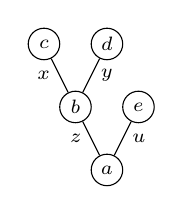
\begin{tikzpicture}[scale=0.8]
    % set up the nodes
    \node (E)[circle,draw=black,minimum size=4mm,inner sep=0.1mm] at (0,0) {\scriptsize $a$};
    \node (F) [circle,draw=black,minimum size=4mm,inner sep=0.1mm] at (-0.5,1) { \scriptsize $b$};
    \node (A) [circle,draw=black,minimum size=4mm,inner sep=0.1mm] at (0.5,1) {\scriptsize $e$};
    \node (Asubt) [circle,draw=black,minimum size=4mm,inner sep=0.1mm] at (-1,2) {\scriptsize  $c$};
    \node (P) [circle,draw=black,minimum size=4mm,inner sep=0.1mm] at (0,2) {\scriptsize $d$};
    % draw arrows and text between them
    \draw[-] (E)--(F) node  [midway,left] {\scriptsize $z$};
    \draw[-] (E)--(A) node  [midway,right] {\scriptsize $u$};
 \draw[-] (F)--(Asubt) node [midway,left] {\scriptsize $x$};
 \draw[-] (F)--(P) node [midway,right] {\scriptsize $y$};
   \end{tikzpicture}}

&&
\resizebox{2cm}{!}{
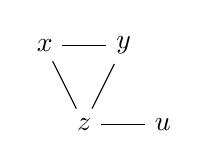
\begin{tikzpicture}
    % set up the nodes
    \node (Z)[] at (-0.5,0) {$z$};
    \node (U)[]  at (0.5,0) {$u$};
    \node (X)[]  at (-1,1) {$x$};
    \node (Y)[]  at (0,1) {$y$};
    % draw arrows and text between them
    \draw[-] (Z)--(U) node  {};
 \draw[-] (Z)--(X) node  {};
 \draw[-] (Z)--(Y) node {};
 \draw[-] (X)--(Y) node {};
   \end{tikzpicture}}
\end{tabular}
\end{center}
An {\em operahedron} is a hypergraph polytope (in fact, a graph associahedron) arising as $\hyper{G}({\cal T})$ for some ${\cal T}$. Its constructs (resp. constructions) are in one-to-one correspondence with the nestings (resp. full nestings)\marginpar{ILLUSTRER} of ${\cal T}$ and allow to give a 
geometrical proof of coherence for categorified non-symmetric operads~\cite{DP15,CLA1}. 

\begin{proposition} Operahedra are contextual.
\end{proposition}
\begin{proof}
It is proved in~\cite{COI}[see Lemma 12] that the connected subsets of $\hyper{G}({\cal T})$ are in bijective correspondence with the subtrees of $\cal T$ having at least two nodes, through a map $E\mapsto  {\cal T}_E$ such that 
$\hyper{G}({\cal T})_E=\hyper{G}({\cal T_E})$. Suppose, say, that $\set{x,y,z}\inc E$ and $\xyz{x}{\hyper{G}({\cal T})_E}{\set{y},\set{z}}$. Then it means on the tree side that after
removing the edge $x$ from ${\cal T}_E$, 
resulting in two disjoint subtrees ${\cal T}_E^1$ 
and ${\cal T}_E^2$ 
of ${\cal T}_E$, we have, say, $y\in{\cal T}_E^1$ and $z\in{\cal T}_E^2$. 
On the other hand, removing $x$ from ${\cal T}$ results in subtrees ${\cal T}^1$ and ${\cal T}^2$, containing ${\cal T}_E^1$ and ${\cal T}_E^2$, respectively. Therefore
 $\xyz{x}{\hyper{G}({\cal T}))}{\set{y},\set{z}}$. And vice-versa.
\end{proof}

Associahedra form a subfamily of operahedra: those obtained from linear trees.  Consider the linear tree

\vspace{-1cm}
\begin{center}
$$\xymatrix @-1.65pc {{\cal L} & = &X \ar @{-}[rr]^{1}&& Y \ar @{-}[rr]^{2}&& Z \ar @{-}[rr]^{3}&& U}
 $$
 \end{center}
 \vspace{-.2cm}
 
 \noindent
 (represented horizontally).  Then $\hyper{G}({\cal L})$ is the associahedron $\hyper{K}^3$. The constructs of
  ${\cal L}$ decorate a pentagon as follows:

%$$
% \xymatrix @-1.65pc {&& 3(2(1)) \ar @{->}[ddll]_{3(\set{1,2})} \ar @{->}[dddrr]^{\set{2,3}(1)}&& \\
% &&&&\\
%3(1(2)) \ar @{->}[dd]^{\set{1,3}(2)} }&&   && \\
% &&&&2(1,3) \ar @{->}[dddll]_{\set{1,2}(3)}\\
%1(3(2)) \ar @{->}[ddrr]^{1(2,3)} &  &\\
% &&&&\\
% &&1(2(3))&&}
%$$
\begin{center}
$$\xymatrix @-1.65pc {&& 3(2(1)) \ar @{->}[ddll]_{3(\set{1,2})} \ar @{->}[dddrr]^{\set{2,3}(1)}&& \\
 &&&&\\
3(1(2))   \ar @{->}[dd]^{\set{1,3}(2)}&&   && \\
 &&&&2(1,3) \ar @{->}[dddll]^{\set{1,2}(3)}\\
 1(3(2)) \ar @{->}[ddrr]^{1(\set{2,3})} &  &\\
 &&&&\\
 &&1(2(3))&&}$$
\end{center}
and are in bijective correspondence with the vertices and edges of Mac Lane's pentagon (cf. Section \ref{preamble-section}). 
  Let us sketch the encoding:
  \begin{itemize}
  \item $(X\otimes_1 Y)\otimes_2 (Z\otimes_3 U)$, where we annotaded the ``compositions'' $\otimes$ with the vertices of $\hyper{K}^3$, can be written $\otimes_2(\otimes_1(X,Y),\otimes_3(Z,U))$ in prefix (or tree) notation. Then we get 
 $2(1,3)$ by removing the leaf nodes of that tree.
 \item $\alpha_{X,Y,Z}\otimes_3 U$ can be interpreted as $(X\otimes_1 Y\otimes_2 Z)\otimes_3 U$ (a non fully parenthesed expression), which likewise 
 translates as $3(\set{1,2})$,where $3(\_)$ makes the job of contextualisation.
 \item Likewise, we can move from
$\alpha_{X,Y\otimes_2 Z,U}$ to $X\otimes_1(Y\otimes_2 Z)\otimes_3 U$ to $\set{1,3}(2)$, where $2$ makes the job of instantiation.
\end{itemize}
\PL{Taking the 4-dimensional associahedron $\hyper{K}^5$ (with vertex set $\set{0,1,2,3,4}$), we get the following instance in context of $\hyper{K}^3=\recrestr{\hyper{K}^5}{\set{1,2,3}}$, i.e. of Mac Lane's condition:
\begin{center}
$$\xymatrix @-1.65pc {&& 4(3(2(1(0)))) \ar @{->}[ddll]_{4(3(\set{1,2}(0)))} \ar @{->}[dddrr]^{4(\set{2,3}(1(0)))}&& \\
 &&&&\\
4(3(1(0,2)))  \ar @{->}[dd]^{4(\set{1,3}(0,2))}&&   && \\
 &&&&4(2(1(0),3)) \ar @{->}[dddll]^{4(\set{1,2}(0,3))}\\
 4(1(0,3(2))) \ar @{->}[ddrr]^{4(1(0,\set{2,3}))} &  &\\
 &&&&\\
 &&4(1(0,2(3)))&&}$$
\end{center}
We recover the (encoding of the) edge 
 $$
 \xymatrix @-2pc {&& ((((X_1\otimes_0 X_2)\otimes_1 Y)\otimes_2 Z)\otimes_3 U)\otimes_4 V \ar @{->}[dddddll]_(.6){(\alpha_{(X_1\otimes X_2),Y,Z}\otimes U)\otimes V\quad} && \\
 &&&&\\
 &&&&\\
  &&&&\\
    &&&&\\
( ((X_1\otimes_0 X_2)\otimes_1 (Y\otimes_2 Z))\otimes_3 U)\otimes_4 V  &&   && \\
\ }
$$
 displayed of Section \ref{preamble-section} as the top left edge above.}

\medskip
Hypercubes provide another example of contextual hypergraphs. 
\begin{proposition} Hypercubes are contextual.
\end{proposition}
\begin{proof}
We first note that the above description of $\hyper{C}_n$ is saturated, and that $(\hyper{C}_n)_{\set{1,\ldots,m}}=\hyper{C}_m$ (if $m\leq n$).
So we have to check that  for all $m\leq n$ and all $i,j,k\leq m$, we have $\xyz{k}{{\hyper{H}_n}}{\set{i,j}}$ iff
$\xyz{k}{{\hyper{H}_m}}{\set{i,j}}$, which follows immediately from the observation that for all $p\geq m$ we have
$\xyz{k}{{\hyper{H}_p}}{\set{i,j}}$ iff $i<k$ and $j<k$.
\end{proof}






